\documentclass[11pt]{article}
\usepackage[margin=1in]{geometry}
\usepackage{graphicx,amsmath,amssymb}
\usepackage{hyperref}
\title{Entropy-Constrained Neutron Stars from a Universal QCD Bound}
\author{[Your Name]}
\date{\today}

\begin{document}
\maketitle

\begin{abstract}
We show that the universal QCD entropy bound $\Delta S_{\rm RG}=9.81\,k_B$ sets a hard ceiling on dense-matter entropy, inducing a density cutoff that determines neutron star maximum masses and tidal deformabilities. Using an entropy-suppressed EOS and TOV sequences, we demonstrate consistency with $2\,M_\odot$ pulsars and GW170817 $\Lambda_{1.4}$ constraints.
\end{abstract}

\section{Framework}
We adopt the four-component entropy model from Papers 1–3 and impose $S(\rho)\le S_{\max}$ with $S_{\max}\in\{8.0,9.81,12.0\}\,k_B$.

\section{Mass–Radius Relations}
Figure~\ref{fig:mr_all} shows M–R curves generated purely from CSV outputs (no fitting). Data files: \texttt{data/mass_radius\_results\_\*.csv}.

\begin{figure}[h!]
\centering
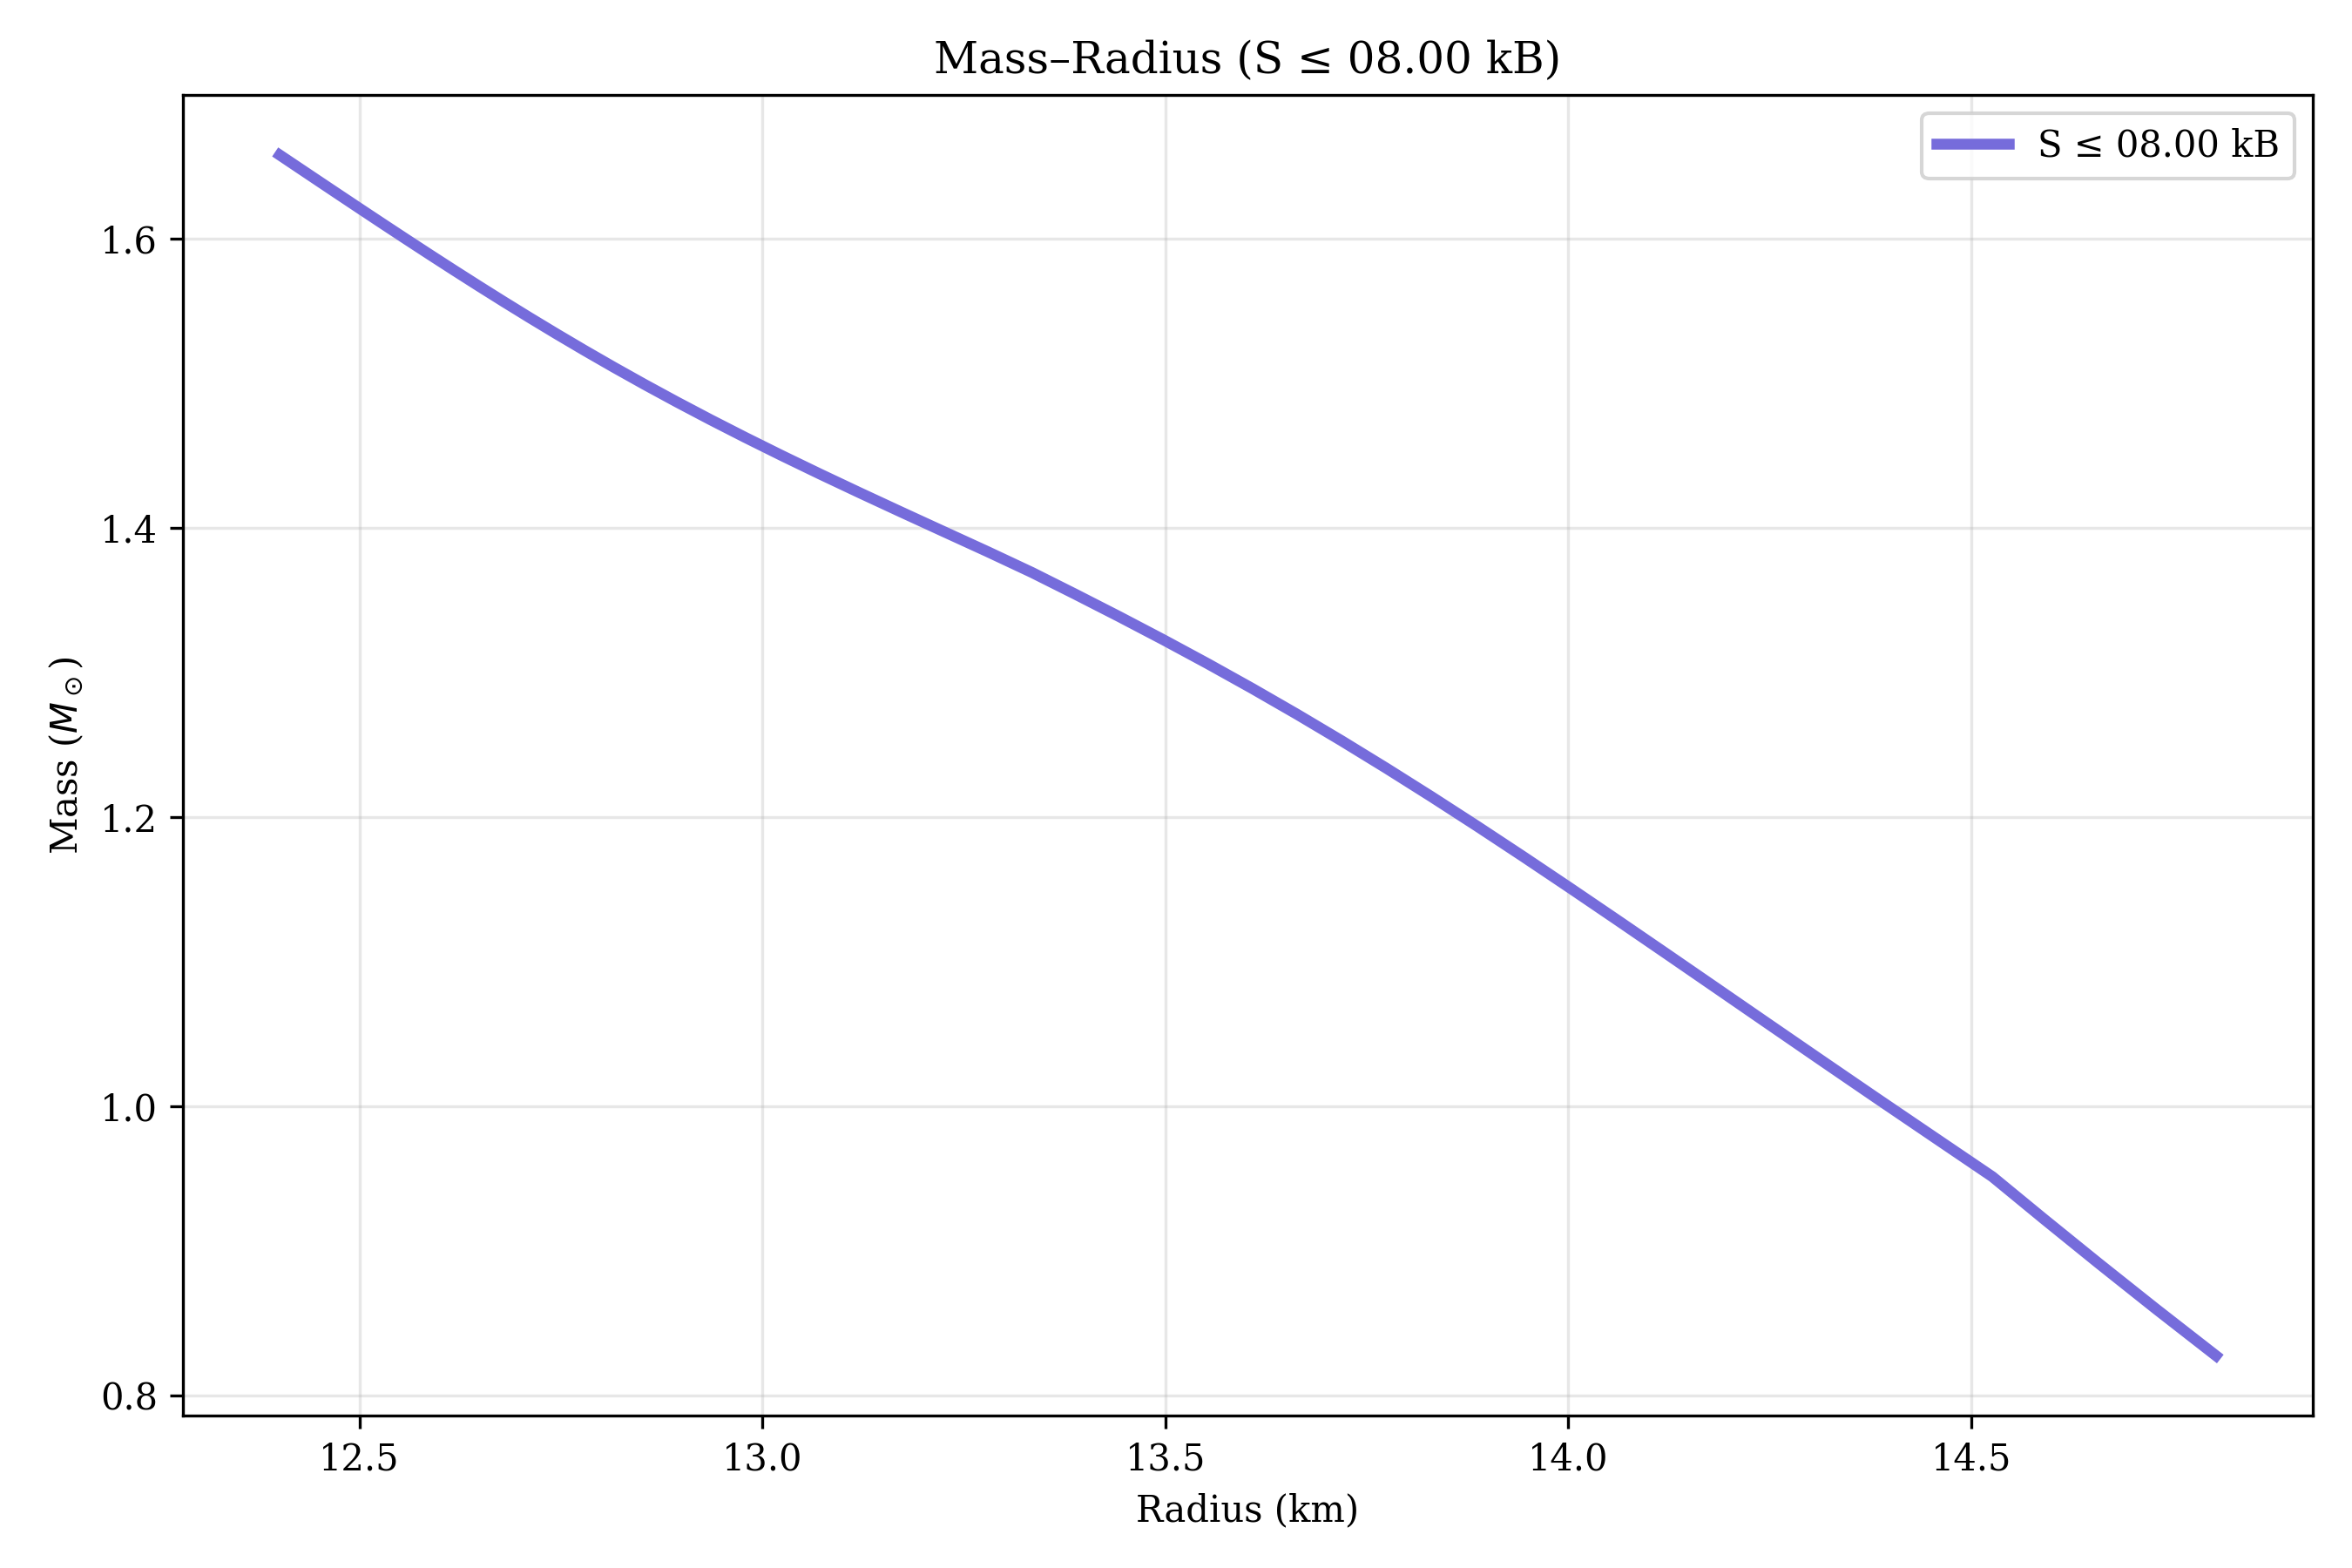
\includegraphics[width=0.32\textwidth]{../figures/mass_radius_curve_08.00kB.png}
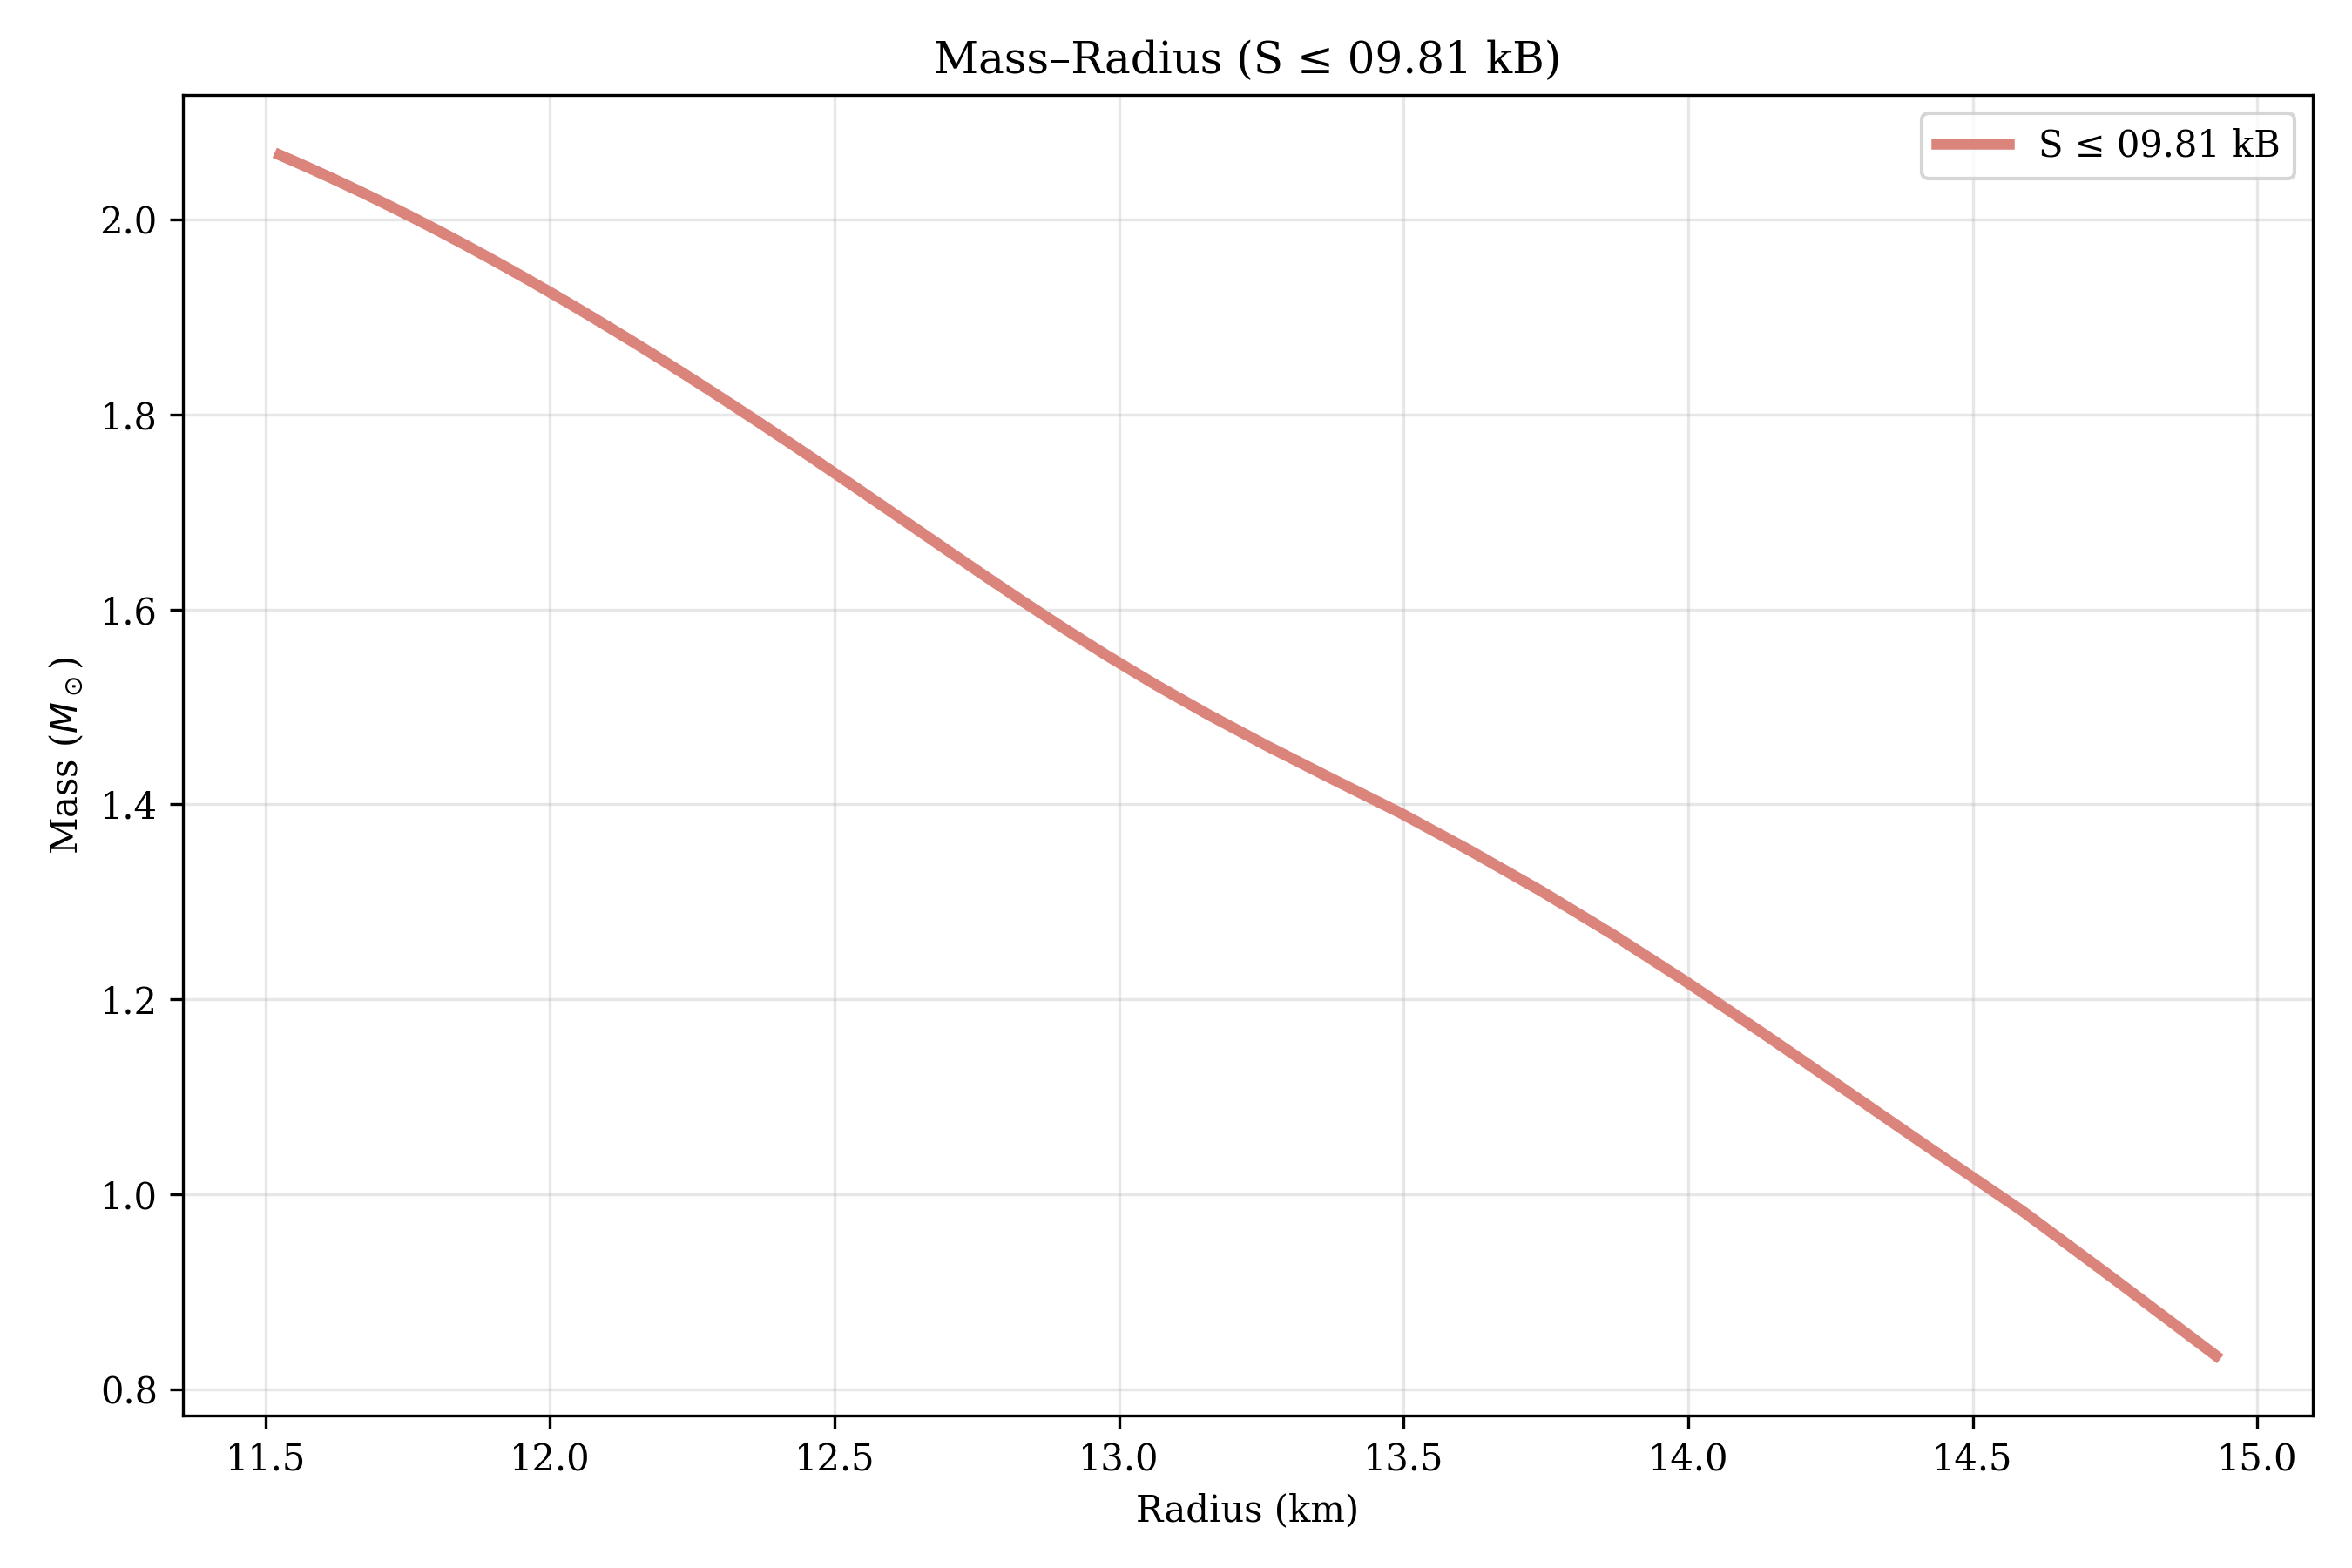
\includegraphics[width=0.32\textwidth]{../figures/mass_radius_curve_09.81kB.png}
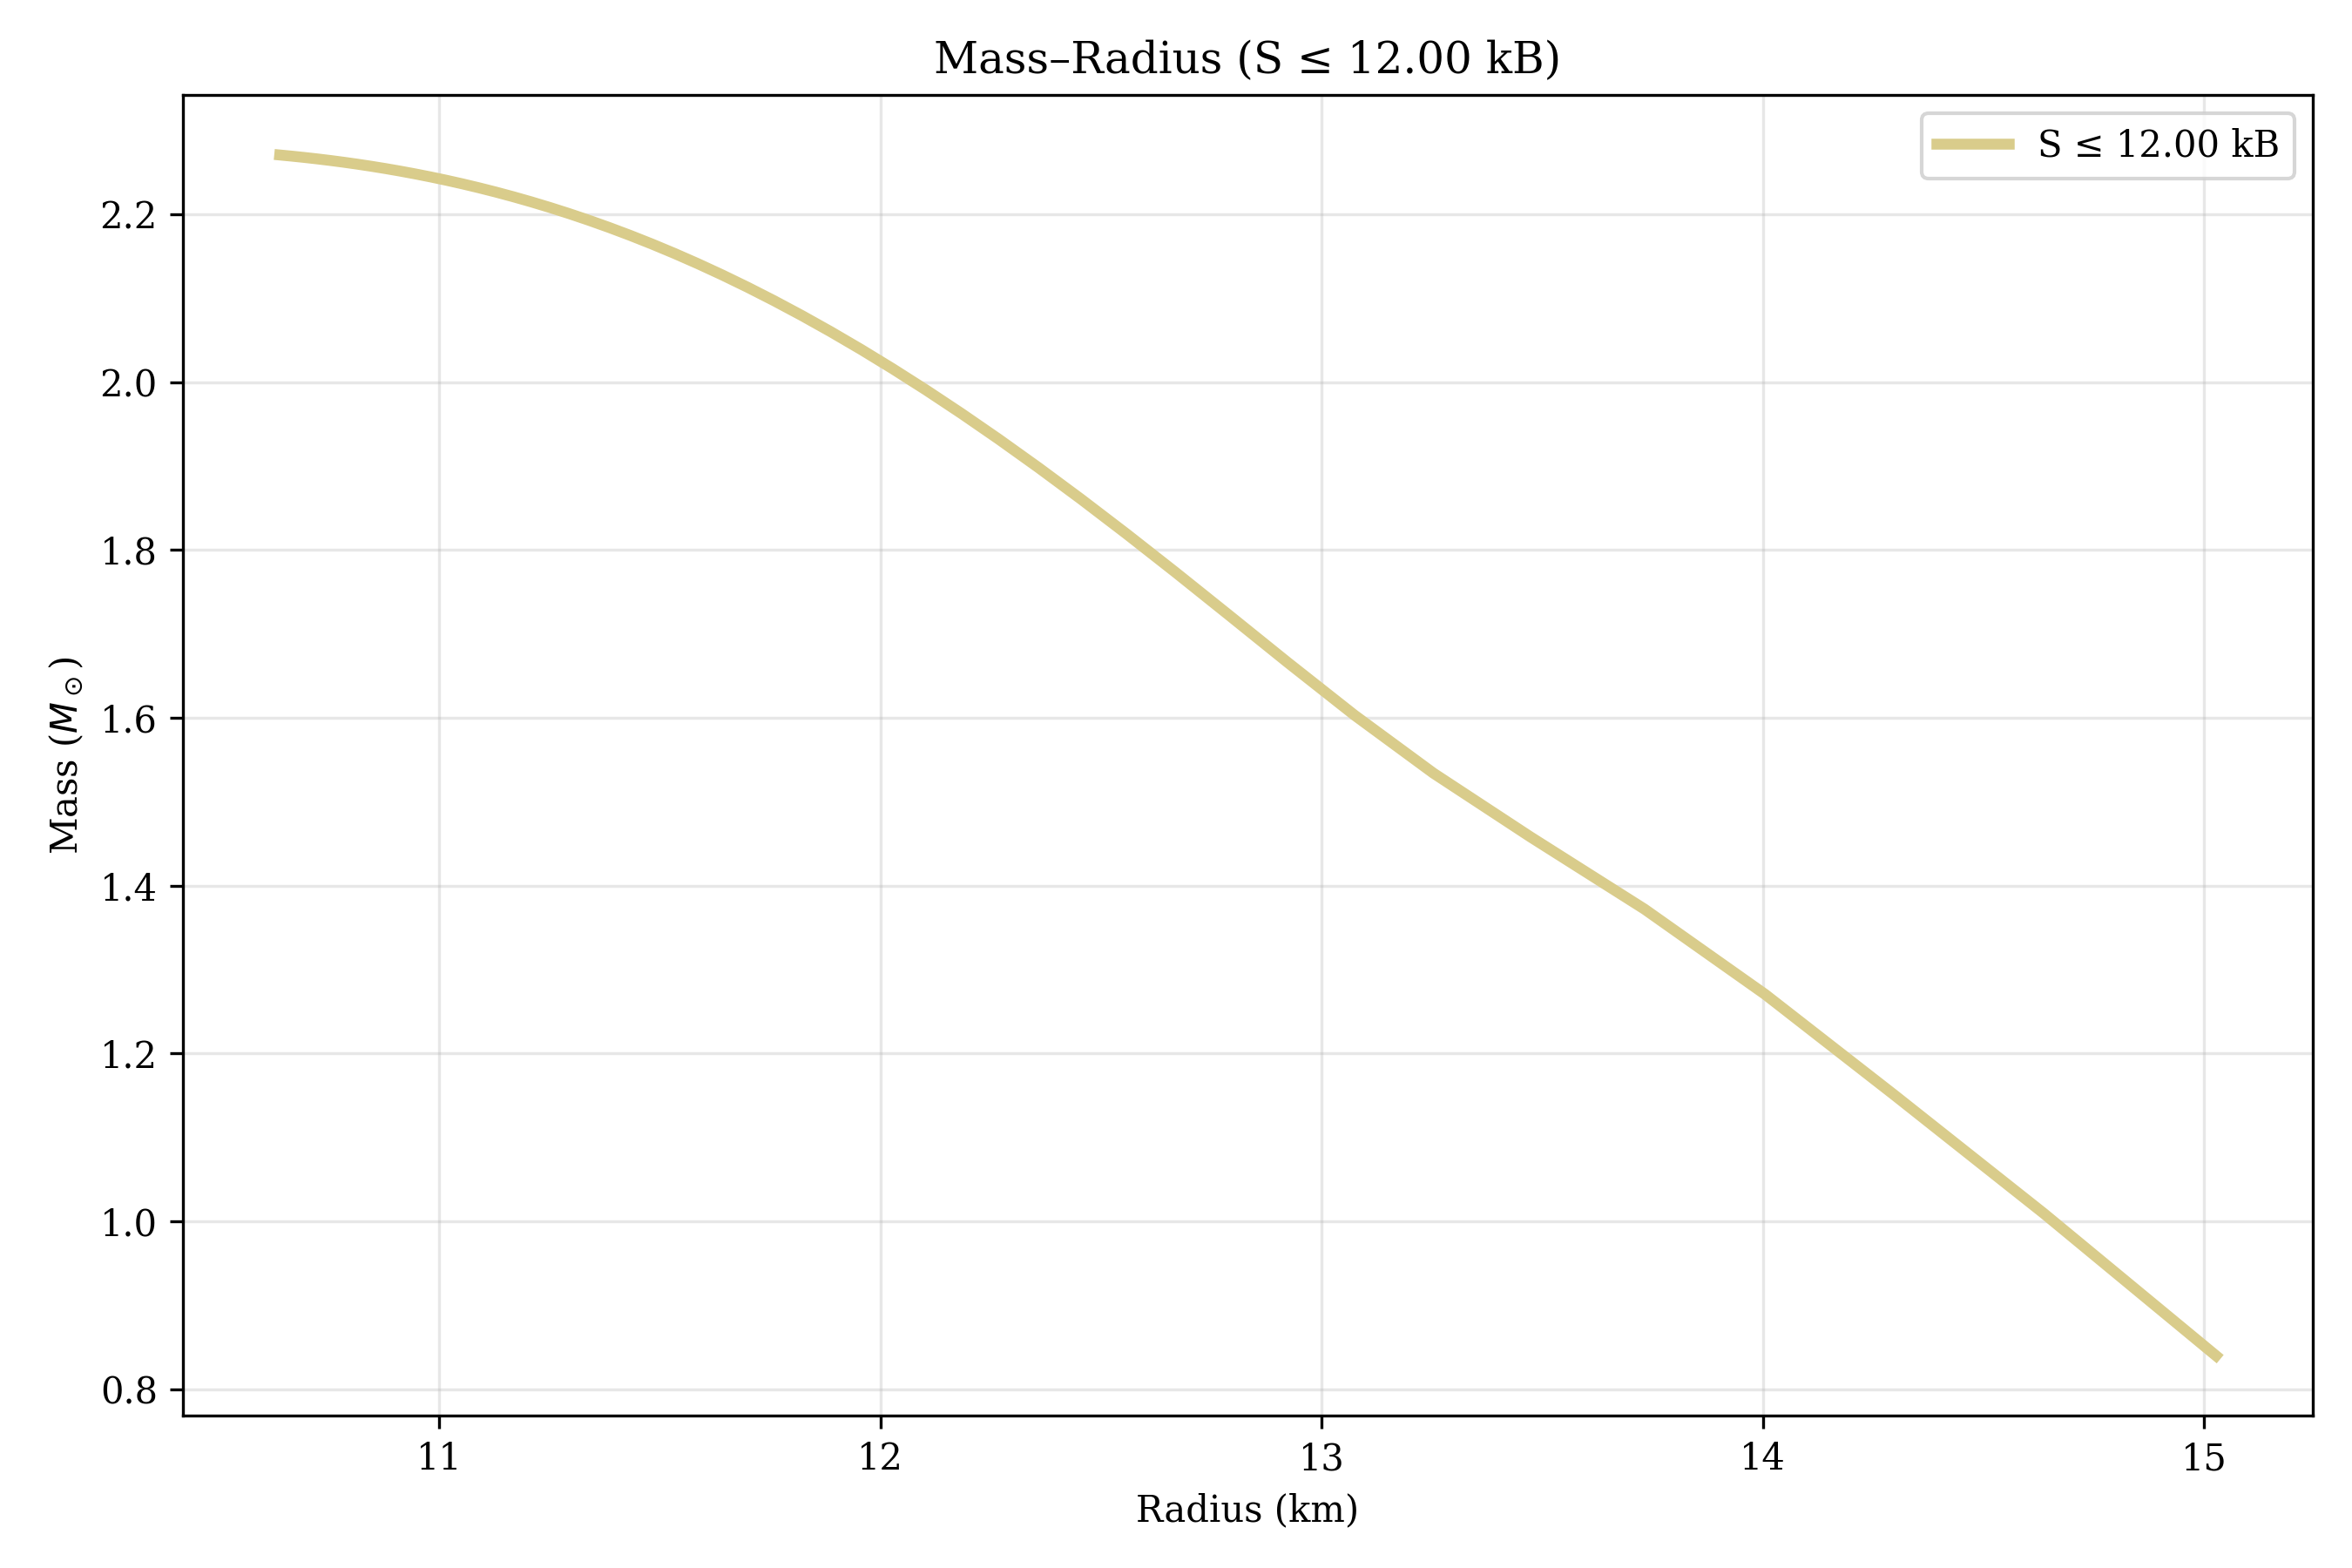
\includegraphics[width=0.32\textwidth]{../figures/mass_radius_curve_12.00kB.png}
\caption{Neutron star mass–radius sequences for entropy caps $S_{\max}=8.0,\,9.81,\,12.0\,k_B$.}
\label{fig:mr_all}
\end{figure}

\section{Tidal Deformability}
Figure~\ref{fig:lambda} shows $\Lambda(M)$ and the GW170817 band.
\begin{figure}[h!]
\centering
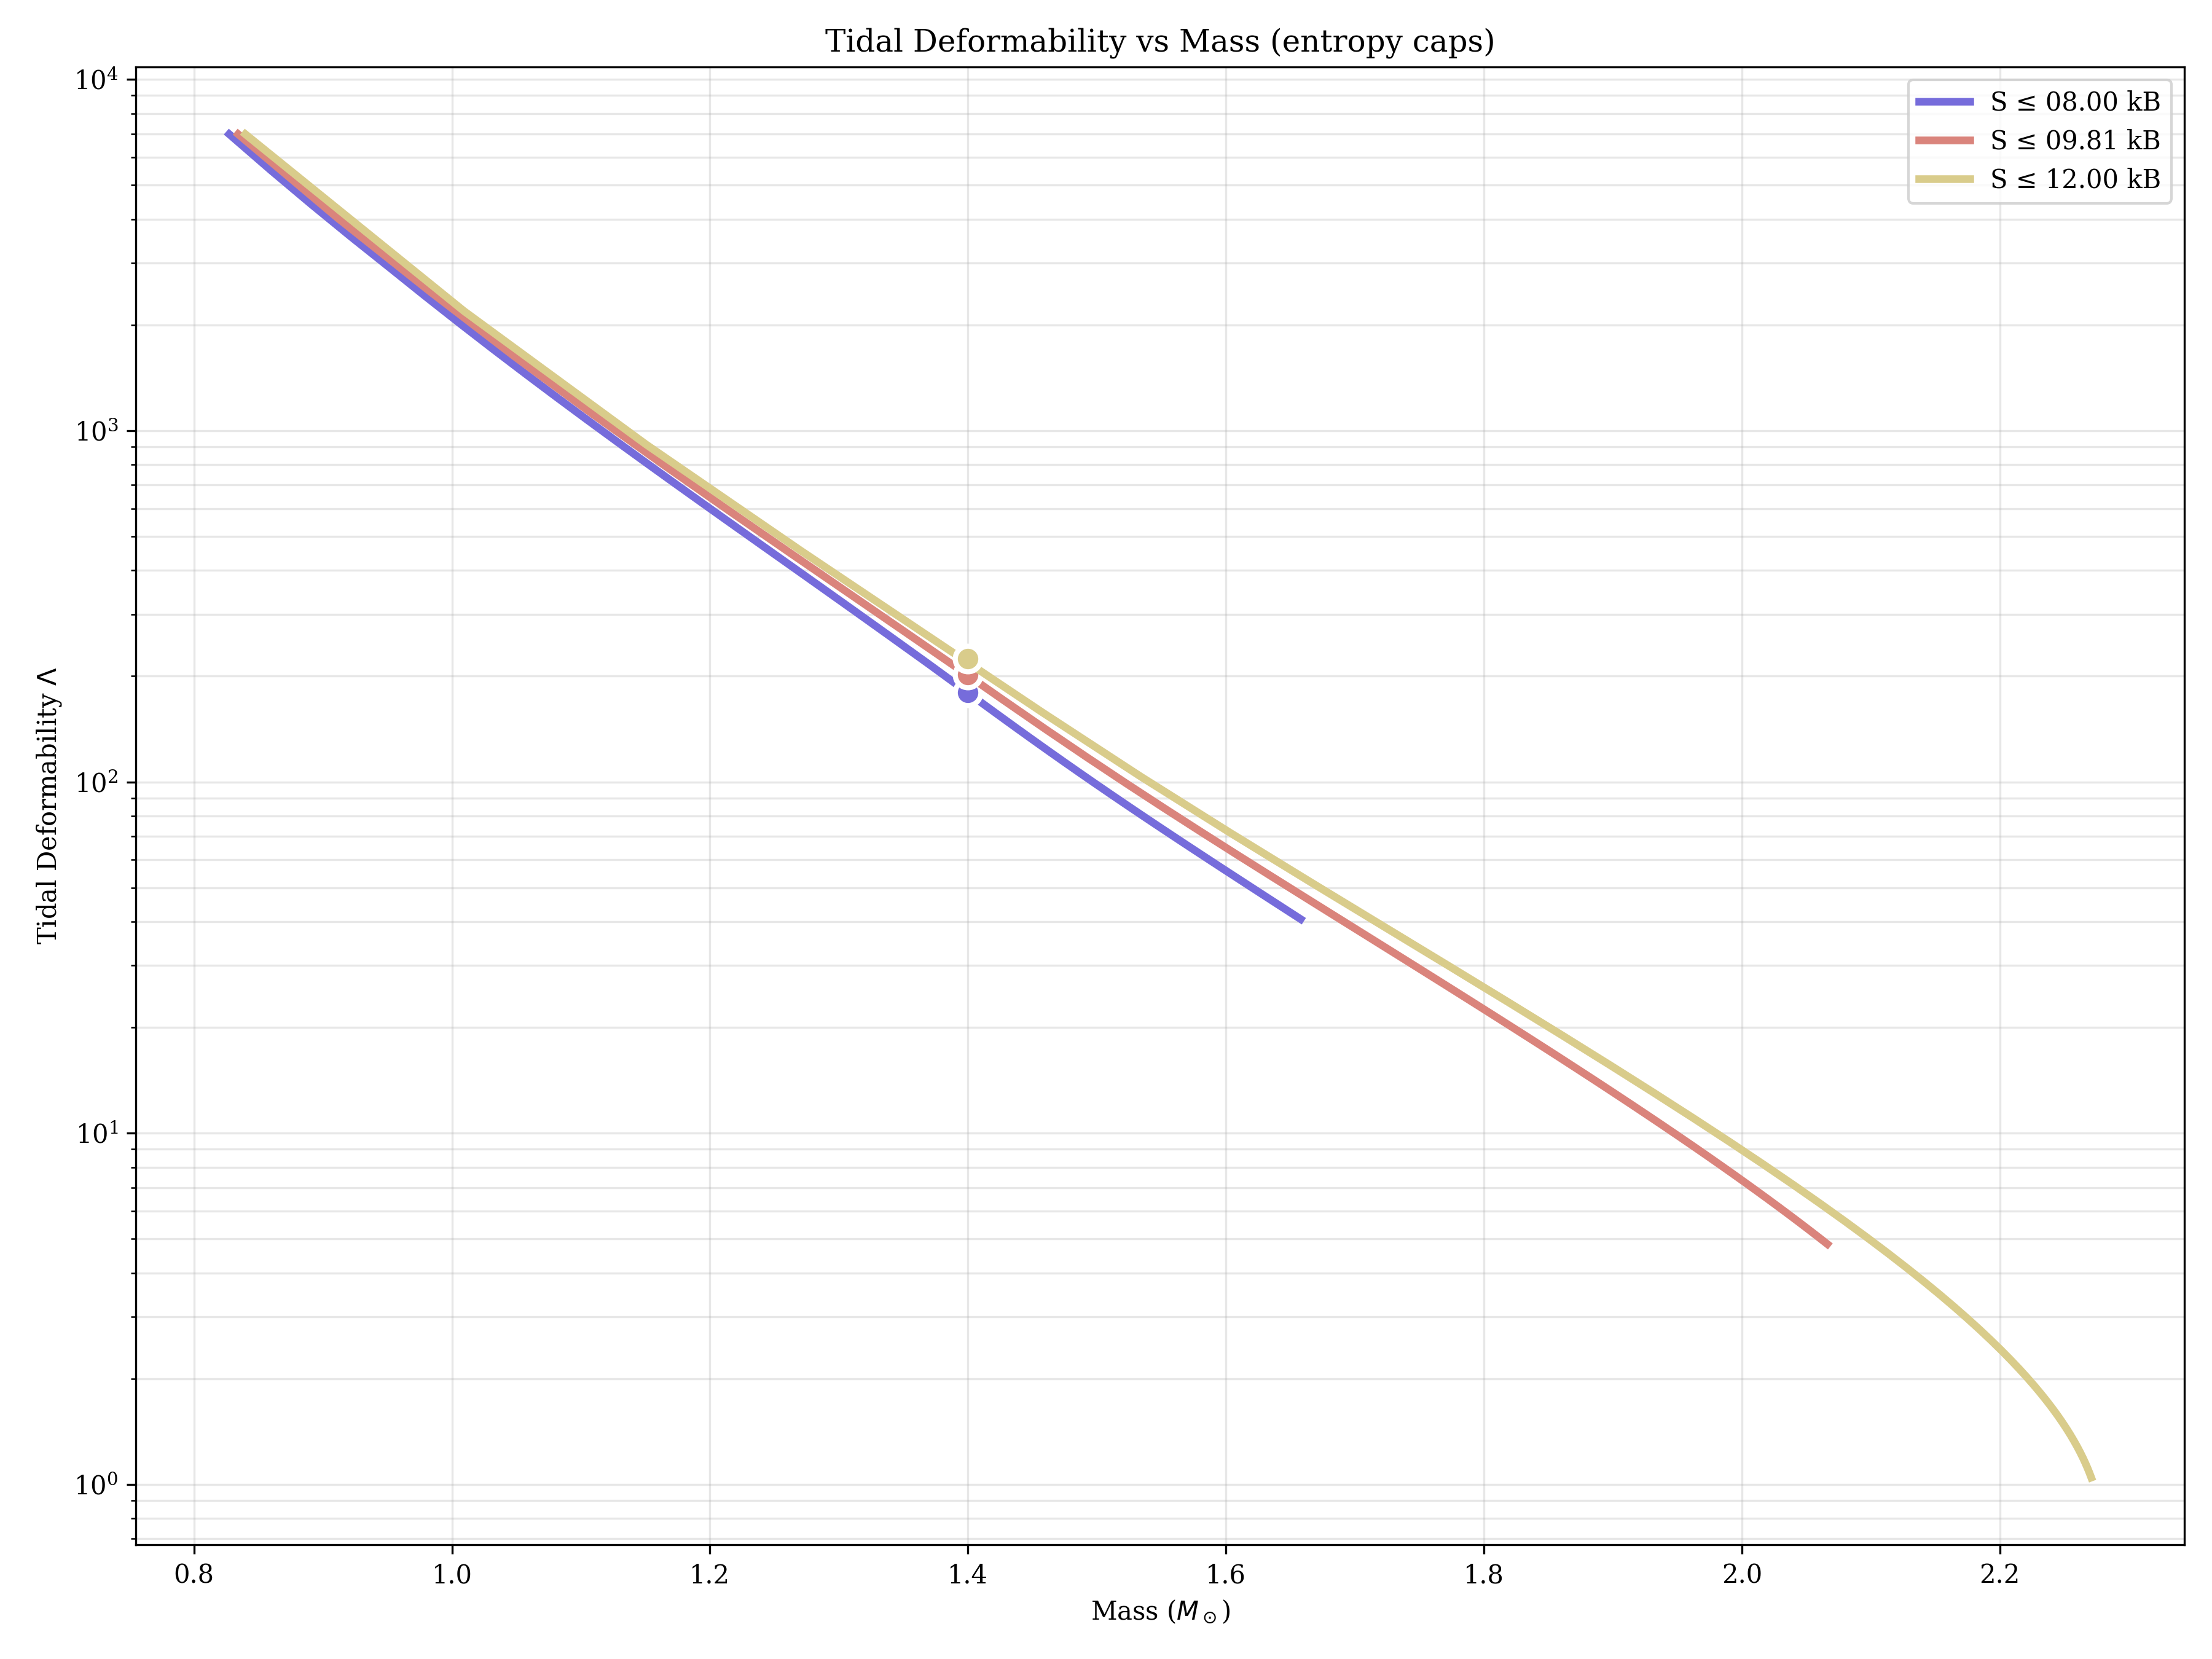
\includegraphics[width=0.6\textwidth]{../figures/appendix_fig_a1.png}
\caption{Tidal deformability $\Lambda(M)$ vs entropy caps; shaded band indicates GW170817 90\%~CI.}
\label{fig:lambda}
\end{figure}

\section{Data Products and Reproducibility}
All CSVs are in \texttt{data/}; figures in \texttt{figures/}; plotting scripts in \texttt{code/}. Run \texttt{./run\_all.sh} to regenerate plots.

\bibliographystyle{unsrt}
\bibliography{refs}
\end{document}
